    % !TEX program = lualatex
\documentclass[8pt]{beamer}

    \usetheme{Madrid}
    \usecolortheme{crane}
    \linespread{1.5}
    
    \usepackage{graphicx}
    %\usepackage{xcolor}
    \usepackage{amsmath}
    \usepackage{physics}
    \usepackage{hyperref}
    \usepackage{slashed}
    \usepackage{siunitx}
    \usepackage{graphicx}
    %\usepackage{enumitem}
    \usepackage{tikz-feynman}
	\usepackage{comment}
	\usepackage{mathrsfs}
    
    \newcommand{\phanitem}{\phantom{\item}}


    \newcommand{\g}{\gamma}
    \renewcommand{\a}{\alpha}
    \renewcommand{\b}{\beta}
    \renewcommand{\t}{\theta}
    \newcommand{\la}{\lambda}
    \newcommand{\p}{\phi}
    \newcommand{\ka}{\kappa}
    \newcommand{\vp}{\varphi}
    \newcommand{\s}{\sigma}
    \newcommand{\G}{\Gamma}
    \newcommand{\lag}{\mathcal{L}}


\title{Meson-meson scattering in 1+1 Dimension% \\and \\Divergence of Klein-Gordon Hydrogen Atom Wave-function Near Origin
}
\author{Yingsheng Huang}
\institute{Institute of High Energy Physics
%\\ \footnotesize (In collaboration with Yu Jia and Rui Yu)
}
\begin{document}
\maketitle

\begin{frame}
	\frametitle{On-going Work}
	\begin{itemize}
		\item Meson-meson scattering amplitude in 1+1 dimension, Guo-ying Chen, Yingsheng Huang, Yu Jia and Rui Yu.
		\item Divergence of Klein-Gordon hydrogen atom wave-function near origin, Yingsheng Huang, Yu Jia and Rui Yu.
	\end{itemize}
\end{frame}

\begin{frame}
	\frametitle{Content}
	\tableofcontents


\end{frame}

\section{1+1-d QCD and 't Hooft model }
\begin{frame}
	\frametitle{\insertsectionhead ('t Hooft, 1974)}
	\begin{eqnarray}
		\mathcal{L}=-\frac{1}{4}G_{\mu\nu}\ _{i}^{\ j}G^{\mu\nu}\ _{j}^{\
		i}+\bar q^{a i}(i\gamma^\mu D_\mu-m_a)q_i^a,
	\end{eqnarray}
	where
	\begin{eqnarray}
		G_{\mu\nu}\ _{i}^{\ j}&=&\partial_{\mu} A_{i}^{\ j}\
		_{\nu}-\partial_\nu A_{i}^{\ j}\ _{\mu}+i g[A_\mu,A_\nu]_{i}^{\
				j},\nonumber\\
		D_\mu q_i^a&=&\partial_\mu q_i^a+ig A_i^{\ j}\ _\mu q_j^a,\nonumber\\
		i,j&=&1,2,...,N_c, \ \ \ \ a=1,2,...,N_f.
	\end{eqnarray}
	Choose light-cone gauge condition
	\begin{equation}
		A_{-}=A^{+}=0,
	\end{equation}
	where
	$A_{-}=\frac{1}{\sqrt{2}}(A^0+A^1)=\frac{1}{\sqrt{2}}(A_0-A_1)$. With this condition gauge field can be solved and transformed into instantaneous potential.

	In
	the light-cone gauge, the nonvanishing components of the field
	strength tensor reads
	\begin{equation}
		G_{+-}=-G_{-+}=-\partial_{-}A_{+},
	\end{equation}


\end{frame}

\begin{frame}
	and the Lagrangian can then be written as
	\begin{equation}
		\mathcal{L}=\frac{1}{2}\mbox{Tr}(\partial_{-}A_{+})^2+\bar
		q^a(i\partial_{+}\gamma_{-}+i\partial_{-}\gamma_{+}-g\gamma_{-}A_{+}-m_a)q^a.
	\end{equation}
	The definition and the algebra for the $\gamma$ matrices read
	\begin{equation}
		\gamma^{+}=\frac{1}{\sqrt{2}}(\gamma^0\pm \gamma^1),\ \
		(\gamma^+)^2=(\gamma^-)^2=0,\ \ \{\gamma^+,\gamma^-\}=2.
	\end{equation}
	The Feynman rules in the light-cone gauge
	\begin{figure}[hbt]
		\begin{center}
			% Requires \usepackage{graphicx}
			\includegraphics[width=10cm]{Feynmanrules.eps}\\
			\caption{Feynman rules in the light-cone gauge.}\label{Feynmanrules}
		\end{center}
	\end{figure}

\end{frame}

\begin{frame}
	Dyson-Schwinger equation in the large $N_c$ limit, no crossed gluons
	\begin{equation}
		S(p)=S_0(p)+i N_c g^2
		S(p)\left[\int\frac{d^2k}{(2\pi)^2}D(p-k)\gamma_{-}S(k)\gamma_{-}\right]S_{0}(p),
	\end{equation}
	\begin{figure}[hbt]
		\begin{center}
			% Requires \usepackage{graphicx}
			\includegraphics[width=8cm,height=2cm]{dressedquark.eps}\\
			\caption{The thin line denotes the free quark propagator and the solid line denotes the dressed quark propagator.}\label{dressedquark}
		\end{center}
	\end{figure}
	Solution to the above equation is found to be
	\begin{eqnarray}
		S(p)=\frac{p_{-}\gamma_{+}}{2p_{+}p_{-}-M^2-\frac{N_c
			g^2}{\pi}\frac{|p_{-}|}{\lambda}+i\epsilon}, \;\;
		M^2=m^2-\frac{N_c g^2}{\pi},
	\end{eqnarray}

	The Bethe-Salpeter equation can be written as
	\begin{align}
		\psi(p,r) & =4iN_c g^2 p_{-}(p_{-}-r_{-})
		[2p_{+}p_{-}-M_1^2-\frac{N_cg^2}{\pi}\frac{|p_{-}|}{\lambda}+i\epsilon]^{-1}\nonumber\\
		          & \times [2(p_{+}-r_{+})(p_{-}-r_{-})-M_2^2-\frac{N_c
			g^2}{\pi}\frac{|p_{-}-r_{-}|}{\lambda}+i\epsilon]^{-1}\nonumber\\&
		\times
		\int\frac{d^2k}{(2\pi)^2}\frac{1}{k_{-}^2}\psi(p+k,r).\label{BS}
	\end{align}
\end{frame}

\begin{frame}
	\begin{figure}[hbt]
		\begin{center}
			% Requires \usepackage{graphicx}
			\includegraphics[width=4cm]{BS.eps}\\
			\caption{The Bethe-Salpeter equation of the bound state. Arrow lines are dressed quark propagators.}\label{BSequation}
		\end{center}
	\end{figure}
	After defining $\varphi(p_{-},r)=\int dp_{+}\psi(p,r)$, one can have
	\small
	\begin{eqnarray}
		\varphi(p_{-},r)&=&i\frac{N_c g^2}{(2\pi)^2}\int dp_{+}
		[p_{+}-\frac{M_1^2}{2p_{-}}-\frac{N_c
			g^2}{2\pi}\frac{sgn(p_{-})}{\lambda}+i\epsilon\cdot sgn(p_{-})]^{-1}\nonumber\\
		&\times&[p_{+}-r_{+}-\frac{M_2^2}{2(p_{-}-r_{-})}-\frac{N_c
			g^2}{2\pi}\frac{sgn(p_{-}-r_{-})}{\lambda}+i\epsilon\cdot sgn(p_{-}-r_{-})]^{-1}\nonumber\\
		&\times&\int dk_{-}\frac{\varphi(p_{-}+k_{-},r)}{k_{-}^2}.
	\end{eqnarray}
	\normalsize
	By taking the $p_{+}$ integral and using
	\begin{equation}
		\int
		dk_{-}\frac{\varphi(p_{-}+k_{-},r)}{k_{-}^2}=\frac{2}{\lambda}\varphi(p_{-},r)
		+P\int dk_{-}\frac{\varphi(p_{-}+k_{-},r)}{k_{-}^2},
	\end{equation}
	where
	$P\frac{1}{k_{-}^2}=\frac{1}{2}(\frac{1}{(k_{-}+i\epsilon)^2}+\frac{1}{(k_{-}-i\epsilon)^2})$,
	one can have the following

\end{frame}

\begin{frame}
	\begin{eqnarray}
		&&[r_{+}-\frac{M_2^2}{2(r_{-}-p_{-})}-\frac{M_1^2}{2p_{-}}-\frac{N_c
			g^2}{\pi \lambda}+i\epsilon]\varphi(p_{-},r)\nonumber\\
		&=&-\frac{N_c
			g^2}{2\pi}\theta(p_{-})\theta(r_{-}-p_{-})\times[\frac{2}{\lambda}\varphi(p_{-},r)+P\int
			dk_{-}\frac{\varphi(p_{-}+k_{-},r)}{k_{-}^2}].
	\end{eqnarray}
	Clearly, the infra-red singularities in both sides cancel with each
	other. After timing the factor $\frac{2\pi}{N_c g^2}r_{-}$ in both
	sides of the above equation and defining the following dimensionless
	quantities
	\begin{equation}
		\frac{2\pi r_{+}r_{-}}{N_c g^2}=\mu^2,\ \ \ \frac{\pi M_{1,2}^2}{N_c
			g^2}=\alpha_{1,2},\ \ \ \frac{p_{-}}{r_{-}}=x,\label{Dless}
	\end{equation}
	we obtain the famous 't Hooft equation
	\begin{equation}
		\mu^2
		\varphi(x)=(\frac{\alpha_{1}}{x}+\frac{\alpha_{2}}{1-x})\varphi(x)-P\int_0^1
		dy\frac{\varphi(y)}{(x-y)^2}.\label{teq}
	\end{equation}
	The solutions to the 't Hooft equation have discrete enginevalues
	$\mu_n^2$, $n=0,1,2,\cdots$. The corresponding enginefunctions
	$\varphi_n$ satisfy the complete and orthogonal relations
	\begin{equation}
		\sum_{n}\varphi_{n}(x)\varphi_{n}^{\ast}(x^\prime)=\delta(x-x^\prime),\
		\ \ \ \ \int_0^1\varphi_{n}^{\ast}(x)\varphi_{m}(x)dx=\delta_{nm}.
	\end{equation}
\end{frame}

\section{Quark-Antiquark Amplitude and Normalized Bound State Wave-function}
\begin{frame}
	\frametitle{\insertsectionhead (Callen, Coote and Gross, 1976)}
	The Bethe-Salpeter equation for the quark-antiquark scattering amplitude can be written as
	\begin{eqnarray}
		\mathcal{T}(p,p^\prime;r)=-\frac{ig^2}{(p_{-}-p_{-}^\prime)^2}
		+i4N_c
		g^2\int\frac{d^2k}{(2\pi)^2}\frac{1}{(k_{-}-p_{-})^2}\tilde{S}(k)\tilde{S}(k-r)\mathcal{T}(k,p^\prime;r),\label{quarkeq}
	\end{eqnarray}

	where $\tilde{S}(p)\gamma_+=S(p)$. This equation has been solved (Callan, Coote and Gross, 1975) and the result is
	\small
	\begin{eqnarray}
		\mathcal{T}(x,x^\prime;r)
		&=&-\frac{ig^2}{r_{-}^2(x-x^\prime)^2}+\sum_{n}\frac{i}{r^2-r_{n}^2}\left\{\varphi_{n}(x)\frac{g^2}{|r_{-}|}
		\sqrt{\frac{N_c}{\pi}}\left[\theta(x(1-x))\frac{2|r_{-}|}{\lambda}+\frac{\alpha_1}{x}+\frac{\alpha_2}{1-x}-\mu_{n}^2\right]\right\}\nonumber\\
		&&\times\left\{\varphi_n^{\ast}(x^\prime)\frac{g^2}{|r_{-}|}\sqrt{\frac{N_c}{\pi}}
		\left[\theta(x^\prime(1-x^\prime))\frac{2|r_{-}|}{\lambda}+\frac{\alpha_1}{x^\prime}+\frac{\alpha_2}{1-x^\prime}-\mu_n^2\right]\right\},\label{qqamp}
	\end{eqnarray}
	\normalsize
	where $x=\frac{p_-}{r_-},\ \  x^\prime=\frac{p_-^\prime}{r_-}.$

\end{frame}

\begin{frame}
	\begin{figure}[hbt]
		\begin{center}
			% Requires \usepackage{graphicx}
			\includegraphics[width=10cm]{quarkscattering.eps}\\
			\caption{The Bethe-Salpeter equation for quark-antiquark scattering amplitude.}\label{quarkscattering}
		\end{center}
	\end{figure}
	The
	amplitude has infinite poles at $r^2=r_n^2,\ n=0,1,2\cdots$.
	Physical interpretation of the above solution is clear, the
	summation of the t-channel multi-gluon exchange is equivalent to the
	summation of the s-channel quark-antiquark bound state exchange. The
	residue of the pole gives the normalized bound-state wave function
	\begin{equation}
		\Phi^{1,2}_{n}(x)=\varphi_{n}(x)\frac{g^2}{|r_{-}|}
		\sqrt{\frac{N_c}{\pi}}\left[\theta(x(1-x))\frac{2|r_{-}|}{\lambda}+\frac{\alpha_1}{x}+\frac{\alpha_2}{1-x}-\mu_{n}^2\right].
	\end{equation}
	Function $\Phi^{1,2}_n(x)$ can also be interpreted as the transition
	amplitude between the bound state and the quark pair.

	This so-called form factor serves as an external state and link between bound state and quarks in our amplitude calculation.
\end{frame}


\section{Meson-meson scattering amplitude}
\begin{frame}
	\frametitle{\insertsectionhead (Gou-ying Chen and Rui Yu)}
	For process $A(q^a\bar q^b)+B(q^c\bar q^a)\rightarrow C(q^a\bar
		q^b)+D(q^c\bar q^a)$ (where $a,b,c$ are different flavor indexes), the amplitude reads
	\begin{align*}
		  & i\mathcal{M} =(1+\mathcal{C})i\mathcal{M}_0,\nonumber          \\
		  & i\mathcal{M}_0 =\theta(\omega_2-\omega_1)i4g^2\omega_1\int_0^1
		dx\int_0^1
		dy\frac{1}{(y\omega_1-\omega_2-x)^2}\varphi_A(\frac{\omega_2-\omega_1+x}{\omega_2-\omega_1+1})\varphi_B(y)
		\varphi_C(x)\varphi_D(\frac{y\omega_1}{\omega_2}),\nonumber
	\end{align*}
	where
	\begin{equation}
		\omega_1=\frac{r_{B-}}{r_{C-}},\ \ \ \omega_2=\frac{r_{D-}}{r_{C-}}.
	\end{equation}
	Here and in the following, we define the operation
	$(A\leftrightarrow C,\ \ B\leftrightarrow D,\ \ \omega_1\rightarrow
		\frac{\omega_2}{1+\omega_2-\omega_1},\ \ \omega_2\rightarrow
		\frac{\omega_1}{1+\omega_2-\omega_1})$ as $\mathcal{C}$. One can
	find that the final expression is infra-red safe, thus we postpone
	$\lambda\rightarrow 0$ in our final expression.
	$A(q^a \bar q^b)+B(q^b\bar
		q^a)\rightarrow C(q^a\bar q^b)+D(q^b\bar q^a) $ reads
	\begin{equation}
		i\mathcal{M}=(1+\mathcal{P})(1+\mathcal{C})i\mathcal{M}_{0}.
	\end{equation}
	where the operation $\mathcal{P}$ is defined as
	$\mathcal{P}=(A\leftrightarrow B,\ \ C\leftrightarrow D,\ \
		\omega_1\rightarrow \frac{1+\omega_2-\omega_1}{\omega_2},\ \
		\omega_2\rightarrow \frac{1}{\omega_2})$.
\end{frame}

\begin{frame}
	\frametitle{Diagrams for the three-flavor processes}
	\begin{figure}[hbt]
		\begin{center}
			% Requires \usepackage{graphicx}
			\includegraphics[width=12cm]{mesonssa.eps}\\
			\caption{Four-body contact interaction part for $A(q^a\bar
					q^b)+B(q^c\bar q^a)\rightarrow C(q^a\bar q^b)+D(q^c\bar q^a)$.
				$r_A,r_B$ are the incoming momenta of A and B respectively, and
				$r_C,r_D$ are the outgoing momenta of C and D respectively.
			}\label{mesonscatteringa}
		\end{center}
	\end{figure}

\end{frame}

\begin{frame}
	\begin{figure}[hbt]
		\begin{center}
			% Requires \usepackage{graphicx}
			\includegraphics[width=10cm]{mesonssaaa.eps}\\
			\caption{The meson exchange part for $A(q^a\bar
					q^b)+B(q^c\bar q^a)\rightarrow C(q^a\bar q^b)+D(q^c\bar
					q^a)$}\label{mesonscatteringaaa}
		\end{center}
	\end{figure}
\end{frame}

\begin{frame}
	\frametitle{Diagrams for the two-flavor processes}

	\begin{figure}[hbt]
		\begin{center}
			% Requires \usepackage{graphicx}
			\includegraphics[width=10cm]{mesonssb.eps}\\
			\caption{Basic diagrams for $A(q^a\bar q^b)+B(q^b\bar q^a)\rightarrow C(q^a\bar q^b)+D(q^b\bar q^a)$.}\label{mesonssb}
		\end{center}
	\end{figure}

\end{frame}

\begin{frame}
	$A(q^a \bar
		q^a)+B(q^a\bar q^a)\rightarrow C(q^a\bar q^a)+D(q^a\bar q^a) $ reads
	\begin{eqnarray}
		i\mathcal{M}
		=(1+\mathcal{R})(1+\mathcal{P})(1+\mathcal{C})i\mathcal{M}_{0}+(1+\mathcal{R})i\mathcal{M}_{1},
	\end{eqnarray}
	where
	\small
	\begin{align*}
		i & \mathcal{M}_{1}                                                    \\
		  & =-(1+\mathcal{Q})\theta(1-\omega_1)i4g^2\int_0^1
		dx P\int_0^1
		dy\frac{\omega_1\omega_2}{[(y-1)\omega_1+(1-x)\omega_2]^2}\varphi_A(\frac{x\omega_2}{1+\omega_2-\omega_1})\varphi_B(y)
		\varphi_C(y\omega_1)\varphi_D(x)\nonumber\\
		  & -(1+\mathcal{C})\theta(\omega_2-\omega_1)i4g^2\int_0^1dx P\int_0^1
		dy\frac{\omega_1}{(y\omega_1-x)^2}\varphi_A(\frac{x+\omega_2-\omega_1}{1+\omega_2-\omega_1})\varphi_B(y)
		\varphi_C(x)\varphi_D(\frac{(y-1)\omega_1+\omega_2}{\omega_2})\nonumber\\
		  &
		-(1+\mathcal{Q}+\mathcal{P}+\mathcal{C})\theta(\omega_2-\omega_1)\theta(\omega_1-1)i\frac{4\pi}{N_c}\int_0^1
		dx\left[2r_{C+}r_{C-}+2r_{D+}r_{C-}+\frac{M_a^2}{x-\omega_1}+\frac{M_a^2}{x-1}\right.\nonumber\\
		  & \left.-\frac{M_a^2}{x-\omega_1+\omega_2} -\frac{M_a^2}{x}\right]
		\times\varphi_A(\frac{x-\omega_1+\omega_2}{1+\omega_2-\omega_1})\varphi_B(x/\omega_1)
		\varphi_C(x)\varphi_D(\frac{x-\omega_1+\omega_2}{\omega_2}),\nonumber
	\end{align*}
	\normalsize
	and
	\begin{align}
		  & \mathcal{R}=(C\leftrightarrow D,\ \ \omega_1\rightarrow
		\frac{\omega_1}{\omega_2},\ \ \omega_2\rightarrow 1/\omega_2),\ \ \ \nonumber\\
		  & \mathcal{Q}=(B\leftrightarrow C,\ \ A\leftrightarrow D,\ \
		\omega_1\rightarrow 1/\omega_1,\ \ \omega_2\rightarrow
		\frac{1+\omega_2-\omega_1}{\omega_1}).
	\end{align}
	The amplitude can be different when the flavour composition is different, which leads to 23 scenarios in total.
\end{frame}

\begin{frame}
	\frametitle{Diagrams for the one-flavor processes}
	\begin{figure}[hbt]
		\begin{center}
			% Requires \usepackage{graphicx}
			\includegraphics[width=8cm]{mesonssc.eps}\\
			\caption{Basic diagrams for $A(q^a\bar q^a)+B(q^a\bar q^a)\rightarrow C(q^a\bar q^a)+D(q^a\bar q^a)$.
				There are also diagrams with clock-wised fermion loop.}\label{mesonssc}
		\end{center}
	\end{figure}

	\begin{figure}[hbt]
		\begin{center}
			% Requires \usepackage{graphicx}
			\includegraphics[width=6cm]{replot.eps}\\
			\caption{Reploting the third diagram in Fig.~\ref{mesonssc}.}\label{replot}
		\end{center}
	\end{figure}





\end{frame}

\iffalse\begin{frame}
	\frametitle{Classification}
	The 2 cases of 4 flavor scatterings are splited int 2 kindes as following.
	\begin{align}
		\left\{
		\begin{aligned}
			  & A(f_1\f_4)+B(f_2\f_1)\r C(f_3\f_4)+D(f_2\f_3) \\
			  & iM_{41}=iM_0
		\end{aligned}
		\right.,
	\end{align}
	\begin{align}
		\left\{
		\begin{aligned}
			  & A(f_1\f_4)+B(f_3\f_2)\r C(f_3\f_4)+D(f_1\f_2) \\
			  & iM_{42}=iM_1\qquad\qquad(f_1,f_2,f_3,f_4)
		\end{aligned}
		\right.,
	\end{align}
\end{frame}\fi



\section{Numerical Calculation}
\begin{frame}
	\frametitle{\insertsectionhead (Yingsheng Huang)}
	The whole process is simple:
	\begin{enumerate}
		\item Solve 't Hooft equation and obtain meson masses (the eigen value) and the corresponding eigen states;
		      \begin{enumerate}[(a)]
			      \item BSW method

			            Best for heavy quark mass, easy to solve, minimum time consumption, large matrix size cause difficulty in calculating amplitude.
			      \item 't Hooft's original method

			            Only for light quark, time consuming, not reliable in high exciting states, small matrix size makes it ideal for amplitude calculation.
		      \end{enumerate}
		\item Put the solution into the corresponding scattering amplitude formula.
	\end{enumerate}
	Numerical difficulties:
	\begin{itemize}
		\item Cauchy principal value integration.

		      The main problem in the process. In other words, it's singularity problem in numerical calculation. This cause problems with light (u, s) quark
		\item Integration accuracy and instability.
	\end{itemize}
\end{frame}

\begin{frame}
	\frametitle{Numerical Results}
	Dimensions

	The unit of mass is $\beta=340MeV$. In this case, the mass of charm quark is $m_c=4.19\beta=1.425GeV$, the mass of strange quark is $m_s=0.749\beta=0.2547GeV$ and the mass of bottom quark is $m_b=13.5565\beta=  GeV$.

	CHARMONIUM	$c\bar c$.



	\begin{minipage}{0.49\linewidth}
		\begin{figure}[H]
			\centering
			\includegraphics[width=2.5 in]{2.eps}
			\caption{Quark mass: 1.425 GeV}
			\label{fig:ccbar2}
		\end{figure}
	\end{minipage}
	\begin{minipage}{0.49\linewidth}
		\begin{figure}[H]
			\centering
			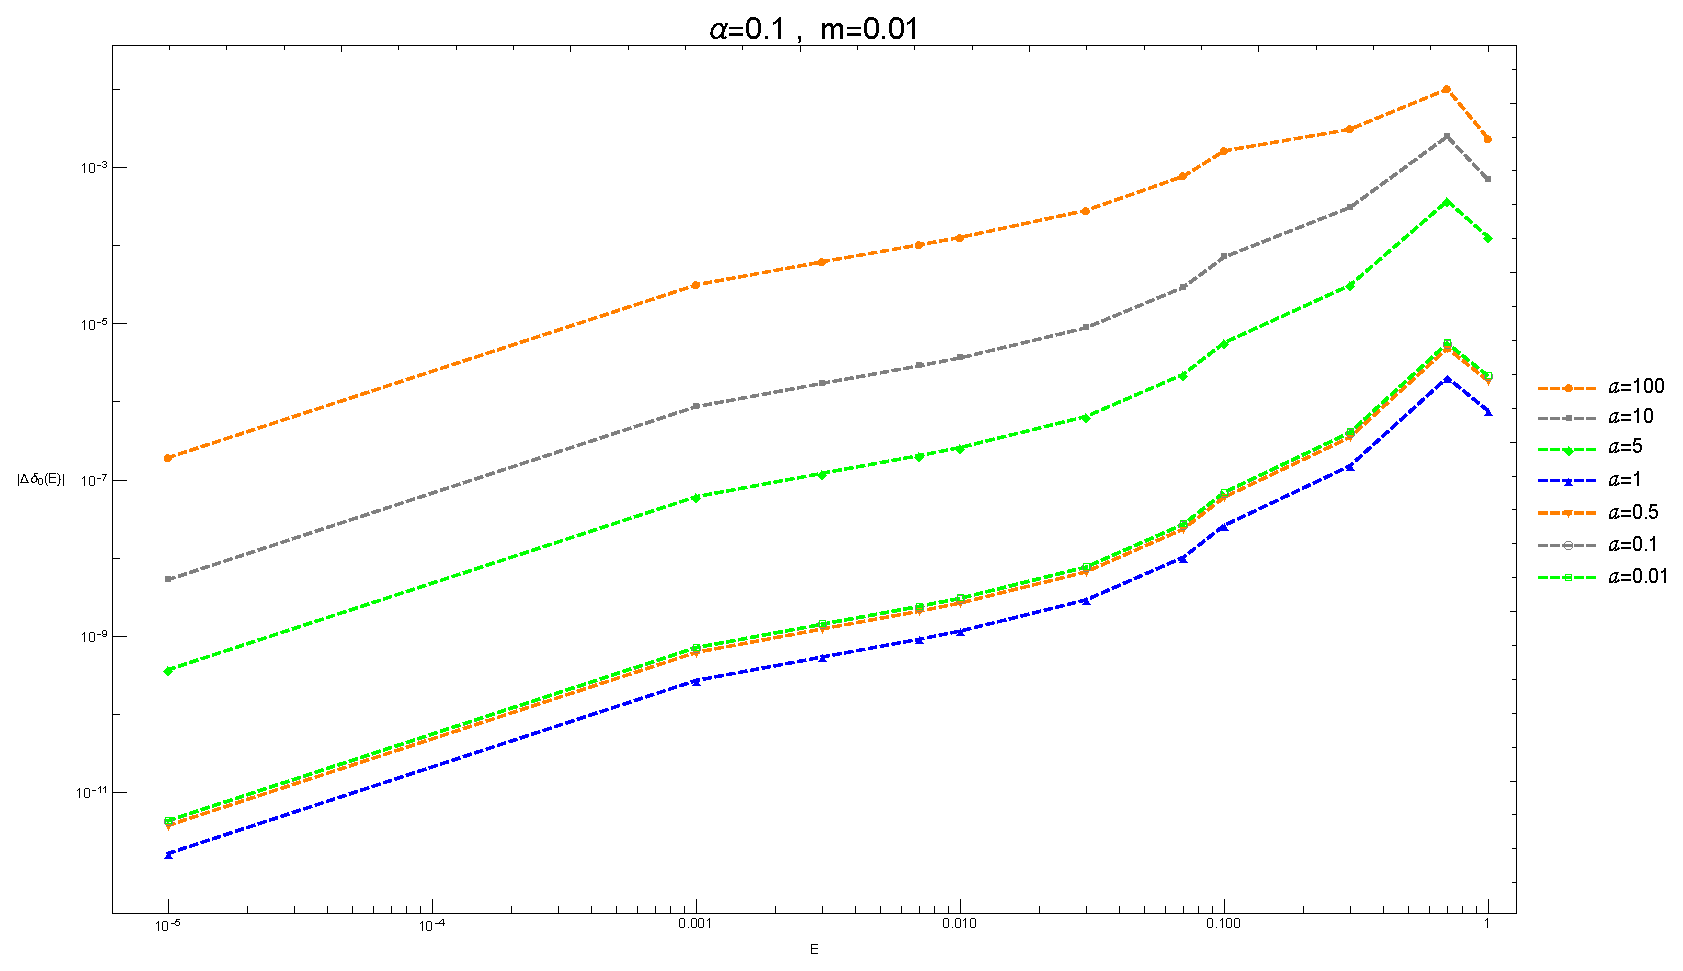
\includegraphics[width=2.5 in]{3.eps}
			\caption{Quark mass: 1.425 GeV}
			\label{fig:ccbar3}
		\end{figure}
	\end{minipage}

\end{frame}

\begin{frame}
	CHARMED, STRANGE MESONS
	$c\bar s$.
	It's $12+21\rightarrow12+21$.

	\begin{minipage}{0.49\linewidth}
		\begin{figure}[H]
			\centering
			\includegraphics[width=2.5 in]{4cs.eps}
			\caption{Quark mass: 1.425 GeV \& 0.2547 GeV }
			\label{fig:csbar}
		\end{figure}
	\end{minipage}
	\begin{minipage}{0.49\linewidth}
		\begin{figure}[H]
			\centering
			\includegraphics[width=2.5 in]{cs.eps}
			\caption{Quark mass: 1.425 GeV \& 0.2547 GeV (HE)}
			\label{fig:csbair2}
		\end{figure}
	\end{minipage}

	BOTTOM MESONS Both $B^{-}(b\bar u)$ and $\bar B^{0}(b \bar d)$.
	$B^-+\bar B^0\rightarrow B^-+\bar B^0$ (TBD).

\end{frame}

\section{Conclusion}
\begin{frame}
	\frametitle{\insertsectionhead}
	\begin{itemize}
		\item Derive 't Hooft equation (Large $N_c$ limit)
		\item Derive normalized bound state wave-function
		\item Calculate amplitudes
		\item Numerical study
		\item We were looking for four-quark state in 1+1-d QCD, and we thought the bump might have something to do with resonance (similar fitting with Breit-Wigner formula was done by Batiz, Pe\~na and Stabler in 2013), and that could mean exotic state.

		      But a cut through the quark line can't produce four quarks, thus four quark intermediate state seems not possible.

		      No concrete conclusion for now.
	\end{itemize}

\end{frame}


\section{Divergence in Relativistic Quantum Mechanics}
\begin{frame}
	\frametitle{\insertsectionhead}
	\begin{minipage}{0.43\linewidth}
		Ground state Klein-Gordon Wave-function with Coulomb potential:
		\begin{align}
			\psi  =\frac{c}{\sqrt{4\pi}}e^{-kr}r^\lambda
		\end{align}
		where
		\begin{align*}
			  & \lambda=-\frac{1}{2}+\sqrt{\frac{1}{4}-Z^2\alpha^2},\; \\&  c=\sqrt{\frac{(2k)^{2(1+\sqrt{\frac{1}{4}-Z^2\alpha^2})}}{\Gamma(2+2\sqrt{\frac{1}{4}-Z^2\alpha^2)})}},\\&    k=\frac{m}{\sqrt{1+\frac{(\frac{1}{2}+\sqrt{\frac{1}{4}-Z^2\alpha^2})^2}{Z^2\alpha^2}}}
		\end{align*}
		expand over $Z\a$ we got logarithmic divergence.
		$$R(r)          \sim-(Z\alpha)^2\log(2m Z \a r)   $$
	\end{minipage}
	\begin{minipage}{0.5\linewidth}
		\begin{figure}
			\centering
			\includegraphics[width=2.8 in]{K-G-fig.pdf}
			\caption{Comparison between Klein-Gordon wavefunction and Schr\"odinger wavefunction, with parameters set at $Z=1$, $\a=0.2$, $m=1$. }
		\end{figure}
	\end{minipage}
\end{frame}

\begin{frame}
	\frametitle{Quantum Mechanics perturbation theory}
	This behavior can be reproduced by simple perturbation theory, with extra power divergence.
	\begin{align}
		H & =H_0+H_{int} ,\;\;H_{int}=H_{kin}+H_{Darwin}+\mathcal{O}(v^6)                                                                                          \nonumber \\
		H & _0=-\frac{\nabla^2}{2m}-\frac{Z\alpha}{r},\ \ \ H_{kin}=\frac{\nabla^4}{8m^3},\ \ \ H_{Darwin}=\frac{1}{32m^4}[-\nabla^2,[-\nabla^2,-\frac{Z\alpha}{r}]]
	\end{align}
	The NLO correrction to wave-function is
	\begin{align}
		\phi^{(1)}=\sum_{n\neq 1}a_{n1}\phi_{n00}^{(0)}+\int d\ka a_{\ka 1}\phi_{\ka00}^{(0)}
	\end{align}
	where $\kappa=\frac{\abs{\vb{k}}}{m Z \a}$ and $\phi_{nlm}^{(0)}$, $\phi_{\ka lm}^{(0)}$ are Schr\"odinger wave-functions in bound state and scattering state.

	The scattering part would cause a divergence when integrating over very-high momentum states, by introducing a hard cutoff $\Lambda$ we can regularize it (Darwin term won't contribute)
	\begin{align}
		R^{(1)}(0)_{kin} & =\int^\frac{\Lambda}{m}d\ka(Z\alpha)^2(\frac{1}{\pi}+\frac{1}{\ka}) \\
		                 & \sim(Z\alpha )^2(\frac{\Lambda}{\pi m}+\log(\frac{\Lambda}{m}))
	\end{align}
\end{frame}

\begin{frame}
	\begin{center}
		\LARGE
		\begin{itemize}
			\item This problem can be dealt with in the framework of QFT!
			\item NRQED, HQET, OPE, Composite Operator, RGE
		\end{itemize}

	\end{center}
\end{frame}

\begin{comment}
\section{Scalar NRQED and HQET}
\begin{frame}
	\frametitle{\insertsectionhead}
	Consider this problem in QFT.

	Describe the nucleus with HQET and the scalar electron with NRQED.

	The Lagrangian is
	\begin{align}
		\lag_{SNRQED+HQET}= & \varphi^*\bqty{iD_0+\frac{\nabla^2}{2m}+\frac{\nabla^4}{8m^3}+\frac{\nabla^6}{16m^5}+\frac{e}{32m^4}\pqty{[\nabla^2,[A_0,\nabla^2]]+[A_0,\nabla^4]}+\mathcal{O}(v^7)}\varphi\nonumber \\&+N^*iD^0N
	\end{align}
	where
	\begin{align*}
		D_{\mu}\varphi=\partial_{\mu}\varphi+ieA_{\mu}\varphi
	\end{align*}
	and
	\begin{align*}
		D_{\mu}N=\partial_{\mu}N-iZeA_{\mu}N
	\end{align*}
	The Feynman rules are thus straight-forward.
\end{frame}

\section{Reproduce divergence in QFT}
\begin{frame}
	\frametitle{\insertsectionhead}
	When discussing heavy quarkonium problem, non-relativistic Coulomb gauge wavefunction can be defined as NRQCD Bethe-Salpeter $Q\bar Q$ wavefunction, evaluated at equal time (Bodwin, Braaten and Lepage, 1995). Given the similar approximation we made here, we could assume the same.
	\begin{align}
		R(\abs{\vb{x}})\propto\mel{0}{\varphi(\vb{x})N(0)}{{}^1H}.\label{wavefunction}
	\end{align}
	We think that the divergence of wavefunction comes from the non-local attribute of operator $\varphi(x)N(0)$ rather than the state $\ket{{}^1H}$ itself, so it can be analyzed by operator product expansion (OPE). We study
	\begin{align}
		\mel{0}{\varphi(\vb{x})N(0)\tilde\varphi(p)\tilde N(k)}{0}=\int\frac{\dd^4 p}{(2\pi)^4}\frac{\dd^4 k}{(2\pi)^4}e^{-ip\cdot y}e^{-ik\cdot z}\mel{0}{\varphi(\vb{x})N(0)\varphi(y)N(z)}{0}.\label{NLME}
	\end{align}
	The dependence of x in this non-local matrix element can also be taken as a regularization scheme and thus the result should be the same as local one (bare)
	$$\mel{0}{\varphi(0)N(0)\tilde\varphi(p)\tilde N(k)}{0}$$
\end{frame}

\begin{frame}
	\frametitle{Local operators: $\mel{0}{\varphi(0)N(0)\tilde\varphi(p)\tilde N(k)}{0}$}
	We do this with dimensional regularization so that all unphysical power divergence will be removed.

	LO is trivial.

	At NLO, there's no logarithmic divergence. (Gamma function has no pole in half-integer points. )
\end{frame}

\begin{frame}
	\frametitle{Non-local operators: $\mel{0}{\varphi(\vb{x})N(0)\tilde\varphi(p)\tilde N(k)}{0}$}
\end{frame}

\begin{frame}
	\frametitle{Renormalization Group Equation}
	We can resum all the logarithms and retain the $r^{Z^2\a^2}$ form. (TBD)

	This process can be done with renormalization group equation, which is the common way to resum large logarithms, i.e. in SCET. Or we can naively calculate and sum all the logarithms the hard way.
\end{frame}

\section{Conclusion}
\begin{frame}
	\frametitle{\insertsectionhead}
\end{frame}
\end{comment}

\begin{frame}
	\begin{center}
		\Huge \usebeamercolor[fg]{frametitle}
		Thanks for your attention!
	\end{center}

\end{frame}

\end{document}